\chapter{SIDIS and the Transverse Structure of the Nucleon}

\section{Introduction}

The spin structure of the nucleon has been of particular interest since the 
EMC~\cite{Ashman:1987hv} measurements implied that the helicity of the 
constituent quarks account for only a fraction of the nucleon spin.  The 
so-called ``spin crisis'' was subsequently confirmed by a number of other 
experiments at CERN~\cite{Adams:1997tq}, SLAC~\cite{Abe:1998wq,Anthony:1999py},
HERA~\cite{Ackerstaff:1999ey,Airapetian:2004zf}, and JLab~\cite{Fatemi:2003yh}.
Possible interpretations of this result include the contribution of the
orbital momentum of quarks and significant polarization of either the strange 
sea (negatively polarized) or gluons (positively polarized).  The 
contributions to the sum rule for the total helicity of the nucleon
include the following:

\begin{equation}
\frac{1}{2} = \frac{1}{2} \sum_q \Delta q^{val} + \Delta q^{sea}
+L_z^{val} + L_z^{sea} + L_z^{glue} + \Delta G,
\label{angmom_sumrule_a}
\end{equation}

\noindent
where $\Delta q$, $L_z$, and $\Delta G$ are respectively the quark helicity, 
the orbital angular momentum of all partons, and the gluon helicity.

Present knowledge about the spin structure of the nucleon comes mainly from 
polarized deep inelastic scattering (DIS). The polarization of the individual 
flavors and anti-flavors were mainly studied using fits to the inclusive data.
Inclusive DIS is sensitive to only the squared charges of the partons, 
and requires additional assumptions ({\it e.g.} an SU(3) symmetric sea), 
which leads to certain ambiguities.  Semi-inclusive deep inelastic scattering
(SIDIS) studies, when a hadron is detected in coincidence with the scattered 
lepton that allows so-called ``flavor tagging'', provide more direct access to 
contributions from various quarks.  In addition, they give access to the 
transverse momentum distributions of quarks, not accessible in inclusive 
scattering.  Azimuthal distributions of final state particles in semi-inclusive 
deep inelastic scattering  provide access to the orbital motion of quarks and 
play an important role in the study of transverse momentum distributions of 
quarks in the nucleon.

Significant progress has been made recently in understanding the role of 
partonic initial and final state interactions~\cite{Brodsky:2002cx,
Collins:2002kn,Ji:2002aa}.  The interaction between the active parton in
the hadron and the spectators leads to gauge-invariant transverse momentum 
dependent (TMD) parton distributions~\cite{Brodsky:2002cx,Collins:2002kn,
Ji:2002aa,Belitsky:2002sm,Boer:2003cm}.  Furthermore, QCD factorization for 
semi-inclusive deep inelastic scattering at low transverse momentum in the 
current-fragmentation region has been established in Refs.~\cite{Ji:2004wu,
Collins:2004nx}.  This new framework provides a rigorous basis to study the 
TMD parton distributions from SIDIS data using different spin-dependent and 
independent observables.  TMD distributions (see Table~\ref{tab1}) describe 
transitions of a nucleon with one polarization in the initial state to a 
quark with another polarization in the final state.

The diagonal elements of the table are the momentum, longitudinal and 
transverse spin distributions of partons, and represent well-known parton
distribution functions related to the square of the leading-twist, light-cone 
wave functions. Off-diagonal elements require non-zero orbital angular 
momentum and are related to the wave function overlap of $L$=0 and $L$=1 Fock 
states of the nucleon~\cite{Ji:2002xn}.  The chiral-even distributions 
$f_{1T}^\perp$ and $g_{1T}$ are the imaginary parts of the corresponding
interference terms, and the chiral-odd $h_1^\perp$ and $h_{1L}$ are the
real parts.  The TMDs $f_{1T}^\perp$ and  $h_{1}^\perp$, which are related to 
the imaginary part of the interference of wave functions for different orbital 
momentum states and are known as the Sivers and 
Boer-Mulders functions~\cite{Sivers:1990fh,Anselmino:1998yz,Brodsky:2002rv,
Collins:2002kn,Ji:2002aa,Belitsky:2002sm}, describe unpolarized quarks in the 
transversely polarized nucleon and transversely polarized quarks in the 
unpolarized nucleon respectively.  They vanish at tree-level in a $T$-reversal 
invariant model ($T$-odd) and can only be non-zero when initial or final state 
interactions cause an interference between different helicity states.  This 
function parameterizes the correlation between the transverse momentum of 
quarks and the spin of a transversely polarized target or the transverse spin 
of the quark, respectively.  They require both orbital angular momentum, as 
well as non-trivial phases from the final state interaction, that survive in 
the Bjorken limit.  Experimental results on the Sivers functions for up and 
down quarks so far are consistent with a heuristic model of up and down quarks 
orbiting  the nucleon in opposite directions.  The most simple mechanism that 
can lead to a Boer-Mulders function is a correlation between the spin of the 
quarks and their orbital angular momentum.  In combination with a final state 
interaction that is on average attractive, already a measurement of the sign 
of the Boer-Mulders function, would thus reveal the correlation between 
orbital angular momentum and spin of the quarks. 

%%%%%%%%%%%%%%%%%%%%%%%%%%%%%%%%%%%%%%%%%%%%%%%%%%%%%%%%%%%%%%%%%%%%%%%%%%%%%
\begin{table}
\begin{center}
\begin{tabular}{|c|c|c|c|} \hline\hline
N/q & U & L & T \\ \hline
 {U} & ${\color{blue} \bf f_1}$   & & ${\color{red} h_{1}^\perp}$ \\
\hline
 {L} & &${\color{green} \bf g_1}$ &    ${\color{red} h_{1L}^\perp}$ \\
\hline
 {T} & ${\color{blue} f_{1T}^\perp} $ &  ${\color{green} g_{1T}}$ &  ${\color{red} \bf h_1}$ \, ${\color{red} h_{1T}^\perp }$ \\
\hline\hline
\end{tabular}
\end{center}
\caption{\small{{Leading-twist transverse momentum-dependent distribution 
functions.  $U$, $L$, and $T$ stand for transitions of unpolarized, 
longitudinally polarized, and transversely polarized nucleons (rows) to 
corresponding quarks (columns).}}
\label{tab1}} 
\end{table}
%%%%%%%%%%%%%%%%%%%%%%%%%%%%%%%%%%%%%%%%%%%%%%%%%%%%%%%%%%%%%%%%%%%%%%%%%%%%%

The impact parameter space displacement of transversely polarized quark 
distributions in an unpolarized target is described by a chirally odd GPD 
\cite{Burkardt:2005hp}, and has recently been calculated for the first time 
in lattice QCD \cite{Gockeler:2005cd,Gockeler:2006zu}. The resulting transverse
flavor dipole moment for transversely polarized quarks in an unpolarized 
nucleon suggests that the Boer-Mulders functions are significantly larger 
than the Sivers functions.  Moreover, consistent with large $N_C$ predictions, 
the displacement of transversely polarized $u$ and $d$ quarks was found to be 
in the same direction, indicating the same sign for the Boer-Mulders functions
for $u$ and $d$ quarks, and suggesting a further enhancement of the
SIDIS asymmetry from the $d$ quark contribution.

Similar quantities arise in the hadronization process.  One particular case 
is the Collins $T$-odd fragmentation function $H_1^{\perp}$ 
\cite{Collins:1992kk} describing fragmentation of transversely polarized 
quarks into unpolarized hadrons.  Parton model analyses 
\cite{Efremov:2002ut,Afanasev:2003ze,Yuan:2003gu,Metz:2004je} of sub-leading 
single-spin asymmetries observed at HERMES 
\cite{Airapetian:1999tv,Airapetian:2006rx} and {\tt CLAS}~\cite{Avakian:2003pk}
lead to the introduction of new twist-3 $T$-odd distribution functions 
\cite{Collins:2004nx,Boer:2003cm}. 

The off-diagonal TMD distributions arise from interference between amplitudes 
with left- and right-handed polarization states, and only exist because of 
chiral symmetry breaking in the nucleon wave function in QCD.  Their study 
therefore provides a new avenue for probing the chiral nature of the partonic 
structure of hadrons.  The universality of the TMD correlation functions has 
been proven, resulting in a sign change for two $T$-odd TMD distributions 
between Drell-Yan and DIS~\cite{Collins:2002kn,Collins:2004nx}, an exciting 
prediction that has to be confirmed by future experiments.

The JLab 12-GeV upgrade will provide the unique combination of wide kinematic 
coverage, high beam intensity (luminosity), high energy, high polarization,
and advanced detection capabilities necessary to study the transverse momentum 
and spin correlations allowing studies of semi-inclusive processes both in the 
target and current fragmentation regions.  The study of the quark 
distributions  in the valence quark region is one of the key objectives of the 
upgrade project~\cite{CDR}.

\section{Present Experimental Results on Spin-Azimuthal Asymmetries}

In recent years, semi-inclusive deep inelastic scattering (SIDIS) has emerged 
as a powerful tool to probe nucleon structure through transverse single spin 
asymmetries (SSAs)~\cite{Airapetian:1999tv,Airapetian:2004tw,Alexakhin:2005iw}.
In contrast to inclusive deep inelastic lepton-nucleon scattering where 
transverse momentum is integrated out, these processes are sensitive to 
transverse momentum scales on the order of the intrinsic quark momentum
$P_T\sim k_\perp$.  Measurements of SSAs in SIDIS provide access to a list of 
novel physics observables including transversity ($h_1$)
\cite{Ralston:1979ys,Jaffe:1991ra}, and the time-reversal odd Sivers 
distribution function ($f_{1T}^\perp$) 
\cite{Sivers:1990fh,Anselmino:1998yz,Brodsky:2002cx,Collins:2002kn,Ji:2002aa}.

For transversely polarized targets, several azimuthal asymmetries already 
arise at leading order.  Four contributions related to the corresponding 
distribution functions were investigated in Refs.~\cite{Collins:1992kk,Mulders:1995dh,Kotzinian:1994dv,Brodsky:2002cx,Ji:2002aa,Kotzinian:1995cz}:

\begin{eqnarray}
\sigma^{\cos\phi}_{LT} &\propto& \lambda_e S_T y (1-y/2) \cos(\phi - \phi_S)\sum_{q,\bar{q}} e^2_q {x g_{1T}^q(x)} {D_1^{q}(z)}, \\
\sigma^{\sin\phi}_{UT}&\propto&             S_T (1-y)\sin(\phi+\phi_S)\sum_{q,\bar{q}} e^2_q {x h_1(x)} {H_1^{\perp q}(z)}  \nonumber  \\
       &+&             S_T (1-y+y^2/2)\sin(\phi-\phi_S)\sum_{q,\bar{q}} e^2_q {x f^{\perp q}_{1T}(x)} {D_1^{q}(z)} \nonumber\\
       &+&             S_T (1-y)\sin(3\phi-\phi_S)\sum_{q,\bar{q}} e^2_q {x h^{\perp q}_{1T}(x)} {H_1^{\perp q}(z)},
\label{sivco} 
\end{eqnarray}

\noindent 
where $\phi$ and $\phi_S$ are the azimuthal angles of the hadron and transverse 
spin in the photon frame, $x,y,z$ define the fractions of the proton momentum
carried by the struck quark, electron momentum carried by the virtual photon.
and the virtual photon momentum carried by the final state hadron, respectively.
$D_1^{q}(z)$ and $H_1^{\perp {q}}(z)$ are the spin-independent and 
spin-dependent fragmentation functions. 

%%%%%%%%%%%%%%%%%%%%%%%%%%%%%%%%%%%%%%%%%%%%%%%%%%%%%%%%%%%%%%%%%%%%%%%%%%%%%
\begin{figure}[tb]
\begin{center}
\vspace{-6.0cm}
\mbox{ 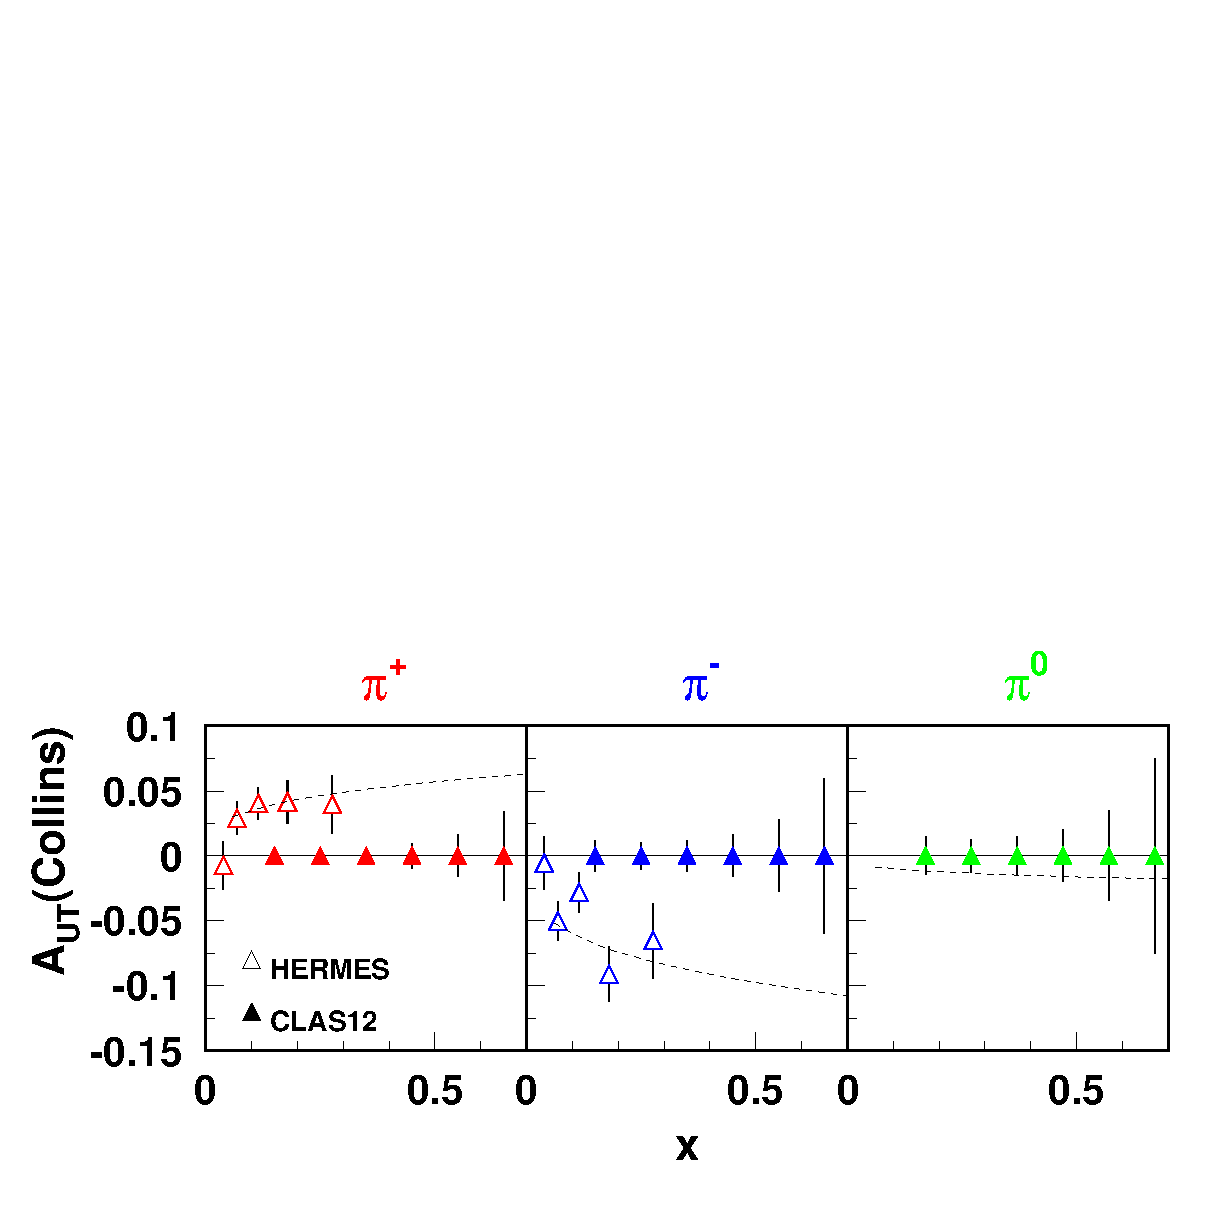
\psfig{file=../sidis/autcollins11.her.eps,height=14cm,width=14.0cm} }
\caption{\small{Projected transverse spin asymmetry from the Collins effect 
($A_{UT}^{\sin(\phi+\phi_S)}$) in single $\pi$ production with {\tt CLAS} at 
11~GeV.}} 
\label{fig:autcol}
\end{center}
\end{figure}
%%%%%%%%%%%%%%%%%%%%%%%%%%%%%%%%%%%%%%%%%%%%%%%%%%%%%%%%%%%%%%%%%%%%%%%%%%%%%

\vspace{0.2cm}\noindent

%%%%%%%%%%%%%%%%%%%%%%%%%%%%%%%%%%%%%%%%%%%%%%%%%%%%%%%%%%%%%%%%%%%%%%%%%%%%
\begin{figure}[tb]
\begin{center}
\vspace{-6.0cm}
\mbox{ 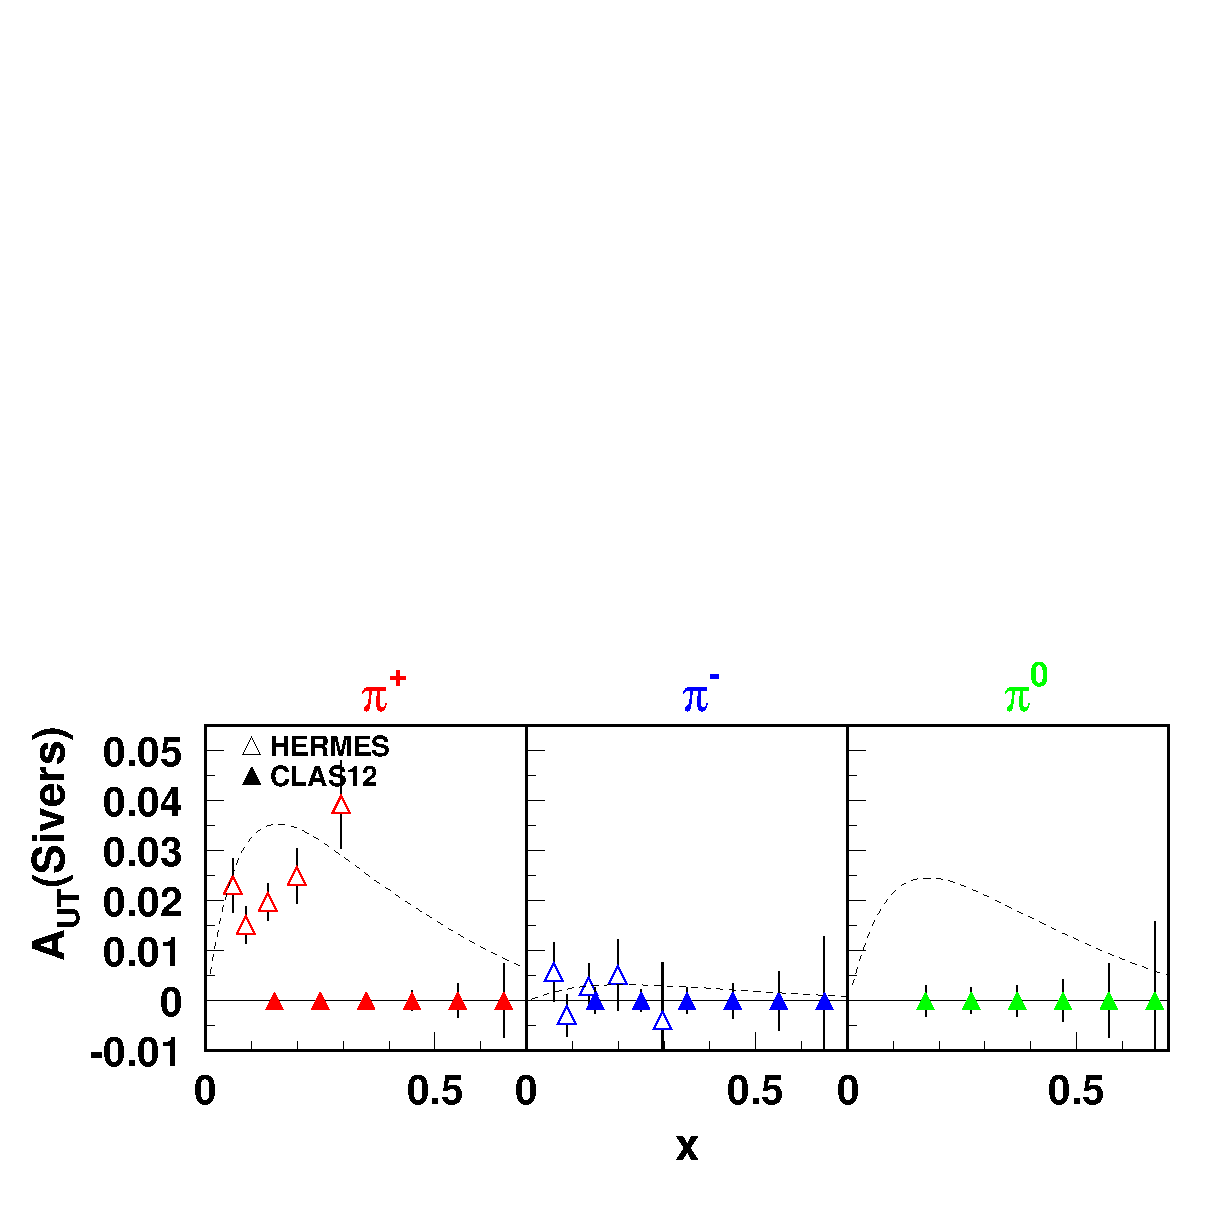
\psfig{file=../sidis/autsivers11.weiss.eps,height=14cm,width=14.0cm} }
\caption{\small{Projected transverse spin asymmetry from the Sivers effect 
($A_{UT}^{\sin(\phi-\phi_S)}$) in single $\pi$ production with {\tt CLAS12} 
at 11~GeV.}}
\label{fig:autsiv}
\end{center}
\end{figure}
%%%%%%%%%%%%%%%%%%%%%%%%%%%%%%%%%%%%%%%%%%%%%%%%%%%%%%%%%%%%%%%%%%%%%%%%%%%%

The leading-twist transversity distribution $h_1$
\cite{Ralston:1979ys,Jaffe:1991ra} and its first moment, the tensor charge, 
are as fundamental for understanding of the spin structure of the nucleon as 
are the helicity distribution $g_1$  and the axial vector charge.  The 
transversity distribution  $h_1$ is charge conjugation odd.  It does not mix 
with gluons and for non-relativistic quarks it is equal to the helicity
distribution $g_1$.  Thus, it probes the relativistic nature of quarks and it 
has a very different $Q^2$ evolution than $g_1$.  The tensor charge is 
reliably calculable in lattice QCD with $\delta \Sigma = \sum_f 
\int_0^1dx(h_1^f - \bar{h_1^f})=0.562 \pm 0.088$ at $Q^2$=2~GeV$^2$, which is 
twice as large as the value of proton axial charge~\cite{Leader:1999rh}.  A 
similar quantity ($\delta \Sigma \approx 0.6$) was obtained in the effective 
chiral quark soliton model~\cite{Kim:1996vk}. 

A detailed study of the $Q^2$ and $x_B$ dependencies as a function of the 
azimuthal angle $\phi$ will allow the separation of contributions from 
different mechanisms.  During the last few years, first results on transverse 
SSAs have become available~\cite{Airapetian:2004tw,Alexakhin:2005iw}. HERMES 
measurements for the first time directly indicated significant azimuthal 
moments generated both by Collins (Fig.~\ref{fig:autcol}) and Sivers 
(Fig.~\ref{fig:autsiv}) effects.

Spin-orbit correlations are also accessible in SIDIS with longitudinally a
polarized target, where they give rise to the Mulders leading-twist 
distribution function $h_{1L}^\perp$. It is related to the real part of
the interference of wave functions for different orbital momentum states,
and describes transversely polarized quarks in the longitudinally polarized 
nucleon.  For a longitudinally polarized target the only azimuthal asymmetry
arising in leading order is the $\sin2\phi$ moment,

\begin{equation}
\sigma^{\sin2\phi}_{UL} \propto S_L 2(1-y)\sin 2\phi\sum_{q,\bar{q}} e^2_q {x h^{\perp q}_{1L}(x)} {H_1^{\perp q}(z)}.
\end{equation}

The physics of $\sigma_{UL}$, which involves the Collins fragmentation 
function $H_1^\perp$ and Mulders distribution function $h_{1L}^\perp$, 
was first discussed by Kotzinian and Mulders in 1996 
\cite{Mulders:1995dh,Kotzinian:1994dv,Kotzinian:1995cz}.  The same 
distribution function is accessible in double polarized Drell-Yan, where it 
gives rise to the $\cos2\phi$ azimuthal moment in the cross section 
\cite{Tangerman:1994eh}.

Measurements of the $\sin2\phi$ SSA \cite{Kotzinian:1995cz}, thus allow the 
study of the Collins effect with no contamination from other mechanisms.  A 
recent measurement of the $\sin 2\phi$ moment of $\sigma_{UL}$ by HERMES 
\cite{Airapetian:1999tv} is consistent with zero.  A measurably large 
asymmetry has been predicted only at large $x$ ($x>0.2$), a region 
well-covered by JLab~\cite{Efremov:2002ut}. 

The kinematic dependence of the SSA for $\pi^+$, measured from the {\tt CLAS} 
EG1 data set at 6~GeV is consistent with predictions~\cite{Efremov:2002ut}. 
The $\pi^+$ SSA is dominated by the $u$-quarks; therefore with some assumption 
about the ratio of unfavored to favored Collins fragmentation functions, it can 
provide a first glimpse of the twist-2 Mulders TMD function.  The distribution 
function $h_{1L}^\perp$ was extracted using the $\pi^+$ target SSA 
\cite{Avakian:2005ps}, which is less sensitive to the unknown ratio of 
unfavored ($d$-quark fragmenting to $\pi^+$) to favored ($u$-quark fragmenting 
to $\pi^+$) polarized fragmentation functions (see Fig. \ref{fig:aul11.sin2}). 
The curve is the result of the calculation by Efremov {\it et al.} 
\cite{Efremov:2002ut}, using $h_{1L}^\perp$ from the chiral quark soliton 
model evolved to $Q^2$=1.5~GeV$^2$.  The extraction, however, suffers from low 
statistics and has a significant systematic error from the unknown ratio of 
the Collins favored and unfavored fragmentation functions, the unknown ratio 
of $h_{1L}^d/h_{1L}^u$, as well as from background from exclusive vector mesons.
Current statistical errors for $\pi^-$, and in particular $\pi^0$, which is 
relatively free of possible higher twist contributions \cite{Afanasev:1996mj},
are large and do not allow strong conclusions from the measured SSAs.  More 
data are required for a statistically significant measurement of the
$\sin2\phi$ moment.

The only leading-twist contribution to the unpolarized target cross section
depending on the azimuthal angle has a term with the Boer-Mulders function 
coupling to the Collins function~\cite{Collins:1992kk}:

\begin{equation}
\sigma^{\cos2\phi}_{UU} \propto 2(1-y)\cos 2\phi\sum_{q,\bar{q}} 
e^2_q {x h^{\perp q}_{1}(x)} {H_1^{\perp q}(z)}.
\end{equation}

The physics of $\sigma^{\cos2\phi}_{UU}$, which involves the Collins 
fragmentation function $H_1^\perp$ and the Boer-Mulders distribution function 
$h_{1}^\perp$, was first discussed by Boer and Mulders in 1998
\cite{Boer:1997nt}.  In recent years, the $\cos 2\phi$ asymmetry in 
leptoproduction was phenomenologically studied using different approximations 
for the Boer-Mulders function 
\cite{Oganesian:1997jq,Gamberg:2003ey,Barone:2005kt}.

Independent information on the Boer-Mulders function 
$h_1^{\perp}(x, \Vec k_T^2)$ can be obtained from the study of the $\cos 2\phi$
azimuthal asymmetry in unpolarized Drell-Yan processes, which has been
measured in $\pi N$ collisions~\cite{Falciano:1986wk,Conway:1989fs}.
In Refs.~\cite{Lu:2004hu,Lu:2005rq} this asymmetry was estimated by computing 
the $h_1^{\perp}$ distribution of the pion and of the nucleon in a quark 
spectator model~\cite{Jakob:1997wg,Bacchetta:2003rz}.  The $\cos 2\phi$ 
azimuthal asymmetry in SIDIS was computed assuming that the $\pi^+$ production 
is dominated by $u$ quarks and using the same distributions
$h_1^{\perp} (x, \Vec k_T^2)$ and $f_1 (x, \Vec k_T^2)$ used in 
Ref.~\cite{Lu:2005rq}.

The calculation of the $\cos 2 \phi$ asymmetry appeared to be in rather good 
agreement for low values of $P_T$ (up to 0.5~GeV) with SIDIS data coming 
from the ZEUS experiment~\cite{Breitweg:2000qi} at large $Q^2$ values 
($0.01<x<0.1$, $0.2<y<0.8$, $0.2<z<1$, $Q^2 > 180$ GeV$^2$) where the 
higher-twist contributions are not expected to be relevant.

It is important to note that both $\pi^+$ and $\pi^-$ azimuthal moments may
have significant contributions from exclusive vector meson production.
The fraction of $\pi^+$ in the single pion sample, coming from exclusive 
$\rho^0$ decays, is somewhat less but still significant at large $z$ and in 
particular for small $x$.  The two pion data from {\tt CLAS12} would allow us
to extract exclusive two pion asymmetries and estimate their contribution to 
the single pion SSA.

\section{TMD Measurements with JLab at 12 GeV}

Projections for target single-spin asymmetry measurements with {\tt CLAS12} 
at 11~GeV are plotted in Figs.~\ref{fig:autcol}-\ref{fig:autsiv}.  The 
projected error bars have been calculated assuming a luminosity of
$5\times 10^{34}$~cm$^{-2}$s$^{-1}$, with an $NH_3$ target polarization of 
85\% and a dilution factor of 0.14, with 2000~hours of data taking.
The asymmetry is integrated over all hadron transverse momenta.

The target single-spin asymmetry from polarized quark fragmentation
extracted for {\tt CLAS12} kinematics at 11~GeV is plotted in 
Fig.~\ref{fig:autcol}.  The estimate was done assuming $h_1 \approx g_1$ and 
an approximation for the Collins fragmentation function from 
Ref.~\cite{Efremov:2002ut}.  Additional cuts were applied on $z$ ($z>0.5$) 
and the missing mass of the $e'\pi^+$ system ($M_X(\pi^+)>1.3$~GeV). 

The extraction of the transversity from $A^{\sin\phi}_{UT}$ could be 
performed using parameterizations for the unpolarized distribution 
functions $u(x)$ and $\bar{d}(x)$ and certain approximations for the 
polarized Collins fragmentation function $H_1^{\perp}$.  The measurement of 
transversity is complicated by the presence of an essentially unknown Collins 
function.  Recently, the Collins function for pions was calculated in a chiral 
invariant approach at a low scale~\cite{Bacchetta:2002tk} and it was shown 
that at large $z$ the function rises much faster than previously predicted 
\cite{Efremov:2002ut,Kotzinian:1999dy} in the analysis using the HERMES data 
on target SSA.  It was also pointed out that the ratio of polarized and 
unpolarized fragmentation is almost scale independent~\cite{Bacchetta:2002tk}.
Significant asymmetry was measured by Belle \cite{Abe:2005zx} indicating that 
the Collins function is indeed large.  The transverse asymmetry measurements 
were performed at HERMES~\cite{Airapetian:2001eg} and COMPASS
\cite{Alexakhin:2005iw}.  The first extraction of the transversity 
distribution has been carried out recently~\cite{Anselmino:2007fs} combining 
$e^+e^-$ and semi-inclusive DIS data~\cite{Airapetian:2004tw}.  The 
statistics, however, are not enough to make statistically significant 
predictions in the valence region, where the effects are large.

Significantly higher statistics from {\tt CLAS12} data, especially in the 
large $\xbj$ region, will enable the extraction of the $\xbj$ and $Q^2$ 
dependencies for different azimuthal moments in a wide kinematic range 
allowing the source of the observed SSA to be revealed and will allow
extraction of the underlying distribution functions.

%%%%%%%%%%%%%%%%%%%%%%%%%%%%%%%%%%%%%%%%%%%%%%%%%%%%%%%%%%%%%%%%%%%%%%%%%%%
\begin{figure}[htbp]
\vspace{7.0cm}
\special{psfile=../sidis/autsivpi0.bnl.eps hscale=70 vscale=65 hoffset=30 voffset=-20}
\caption{\small{Projected transverse spin asymmetry ($A_{UT}^{\sin\phi-\phi_S}$)
in single $\pi^0$ production with {\tt CLAS12} at 11~GeV.  The curves are 
calculated using models for the Sivers function from Efremov {\it et al.}
\cite{Efremov:2004tp}, $F_{1T}=\sum_q^{u,d}e_q^2f_{1T}^{\perp q}$.}}
\label{fig:autsiv1}
\end{figure}
%%%%%%%%%%%%%%%%%%%%%%%%%%%%%%%%%%%%%%%%%%%%%%%%%%%%%%%%%%%%%%%%%%%%%%%%%%%

The measurement of the transverse asymmetry from the Sivers effect (see 
Fig.~\ref{fig:autsiv1}) with $\pi^0$ will provide a model-independent 
extraction of the Sivers function. Furthermore, measurements with proton and 
neutron targets will provide  model-independent information on flavor
partners of the Sivers function.

The transversely polarized target measurements also provide access to the 
leading-twist TMD $g_{1T}^q(x)$ appearing in convolution with the unpolarized
fragmentation function ${D_1^{q}(z)}$ in a $\cos\phi$ moment of the cross 
section.  Significant asymmetries were predicted recently for {\tt CLAS12} 
\cite{Kotzinian:2006dw} providing access also to $g_{1T}^q(x)$, describing 
longitudinally polarized quarks in the transversely polarized nucleon.
Measurements of transverse momenta of final state hadrons in SIDIS with 
longitudinally polarized targets will provide complementary to transverse 
target information, probing the longitudinal nucleon structure beyond the 
collinear approximation.  The $P_\perp$-dependence of the double-spin 
asymmetry, measured for different bins in $z$ and $x$ will provide a test of 
the factorization hypothesis and probe the transition from the non-perturbative 
to perturbative description.  At large $P_T$ ($\Lambda_{QCD}<<P_T<<Q$) the 
asymmetry is expected to be independent of $P_\perp$~\cite{Ji:2004wu}. 
There are indications that the double-spin asymmetry (see 
Fig.~\ref{a1pptdepvszq47x16}) at small $P_T$ tends to increase for $\pi^-$ 
and decrease for $\pi^+$.  A possible interpretation of the $P_T$-dependence 
of the double spin asymmetry may involve different widths of transverse 
momentum distributions of quarks with different flavor and polarization 
\cite{Anselmino:2006yc} resulting from a different orbital structure of quarks 
polarized in the direction of the proton spin and opposite to it 
\cite{Brodsky:1980zm,Brodsky:1994kg}.  This interpretation may demand a 
different width for $d$-quarks than for $u$-quarks, consistent with 
observation from lattice QCD studies of a different spread in transverse 
distances for $d$-quarks compared to $u$-quarks~\cite{Gockeler:2005cd}.
The same effect may be responsible for the relatively large $\cos\phi$ moment
of the double spin asymmetry (see Fig.\ref{a1pptdepvszq47x16}, right panel).

Detailed measurements of $A_{LL}$ and its $\cos\phi$ moment as a function 
of $P_T$ in different bins in $x,z,Q^2$ combined with measurements of
azimuthal moments of the unpolarized cross section proposed for {\tt CLAS12} 
will allow study of the flavor dependence of transverse momentum distributions.

%%%%%%%%%%%%%%%%%%%%%%%%%%%%%%%%%%%%%%%%%%%%%%%%%%%%%%%%%%%%%%%%%%%%%%%%%%%%%
\begin{figure}[htbp]
\vspace{6.8cm}
\special{psfile=../sidis/allpt11.eps hscale=42 vscale=47 hoffset=-5 voffset=-10}
\special{psfile=../sidis/allpt11cos.eps hscale=42 vscale=47 hoffset=240 voffset=-10}
\caption{\small{The double spin asymmetry $A_{LL}$ (left) and its $\cos\phi$ 
moment (right) as a function of the transverse momentum of hadrons, $P_T$,  
averaged in the $0.4<z<0.7$ range.}}
\label{a1pptdepvszq47x16}
\end{figure}
%%%%%%%%%%%%%%%%%%%%%%%%%%%%%%%%%%%%%%%%%%%%%%%%%%%%%%%%%%%%%%%%%%%%%%%%%%%%%

Projections for the resulting kinematic dependence of the leading-twist SSA  
are shown in Fig.~\ref{fig:aul11.sin2}.  Calculations were done using 
$h_{1L}^\perp$ from the chiral quark soliton model evolved to 
$Q^2$=1.5~GeV$^2$~\cite{Efremov:2002ut}, $f_1$ from GRV95~\cite{Gluck:1995yr}, 
and $D_1$ from Kretzer, Leader, and Christova~\cite{Kretzer:2001pz}. Three 
different curves correspond to $H_1^{\perp u\rightarrow \pi^+}/
H_1^{\perp u\rightarrow \pi^-}=0,-1.2,-5$~\cite{Efremov:2004hz}. Corresponding 
projected error bars for the Mulders TMD parton distribution are shown
in Fig.~\ref{fig:aul11.sin2}.  An important ingredient for the estimates are 
so-called ``Lorentz-invariance relations'' that connect $h_{1L}^{\perp}$ with 
$h_1$~\cite{Mulders:1995dh}.  Meanwhile these relations are known not to be 
valid exactly~\cite{Goeke:2003az,Goeke:2005hb}.  It is of importance to find
out experimentally to which extent such relations can provide useful 
approximations, or whether they are badly violated, since there is little 
theoretical intuition on that point.

%%%%%%%%%%%%%%%%%%%%%%%%%%%%%%%%%%%%%%%%%%%%%%%%%%%%%%%%%%%%%%%%%%%%%%%%%%%%%
\begin{figure}
\vspace{-2.0cm}
\begin{tabular}{cc}
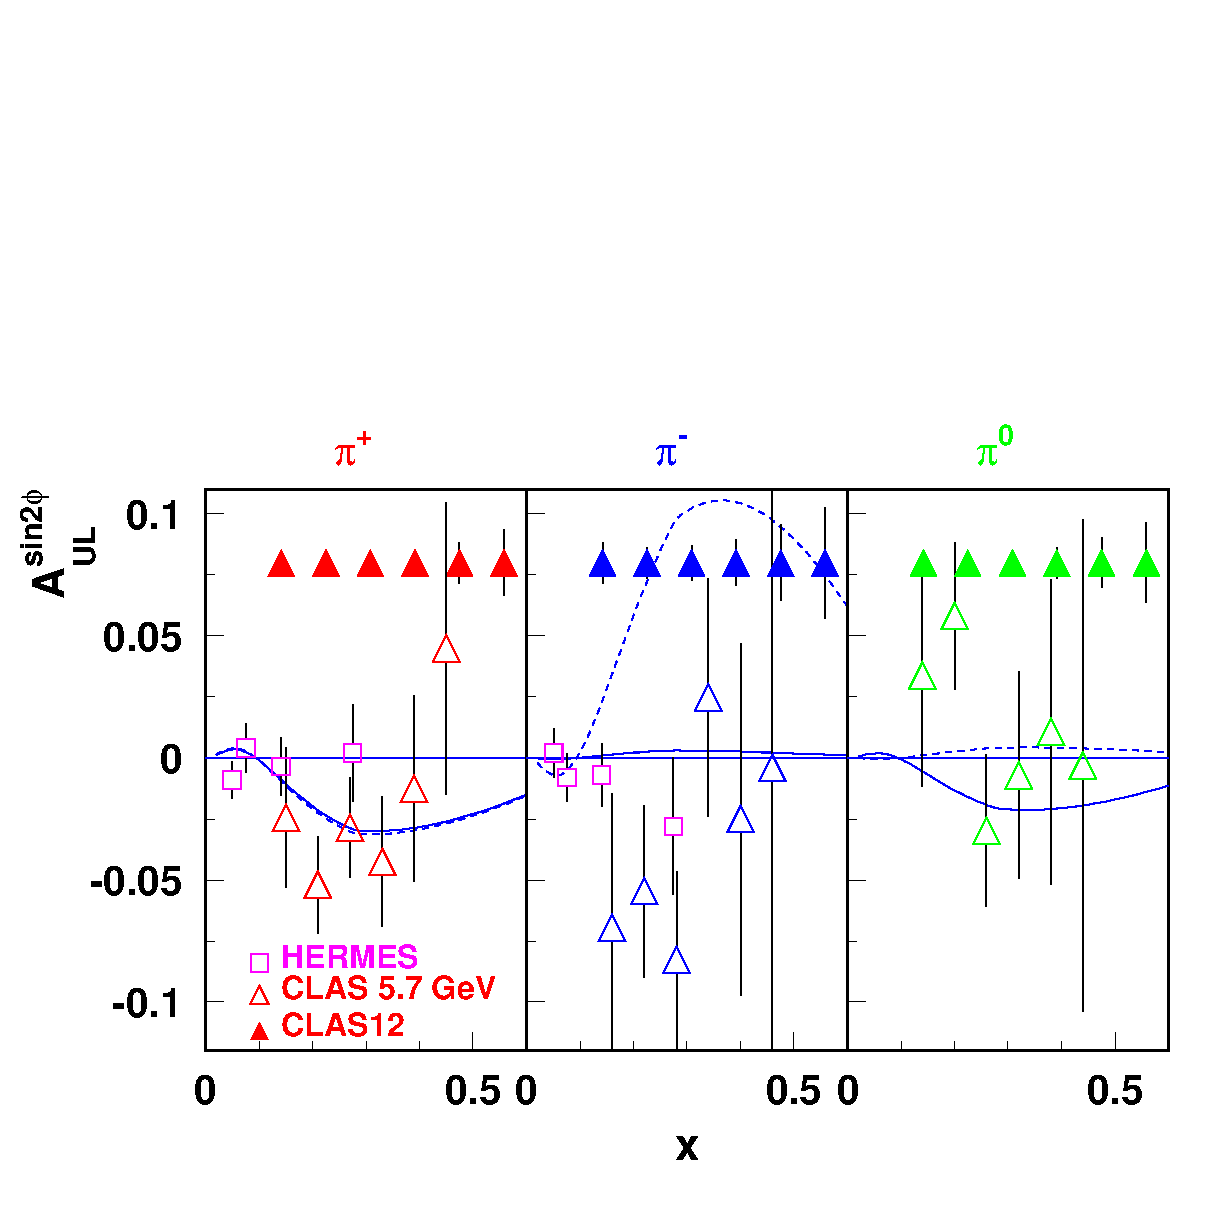
\includegraphics[height=.4\textheight,width=0.45\textwidth]{../sidis/aul11.sin2.eps}
&
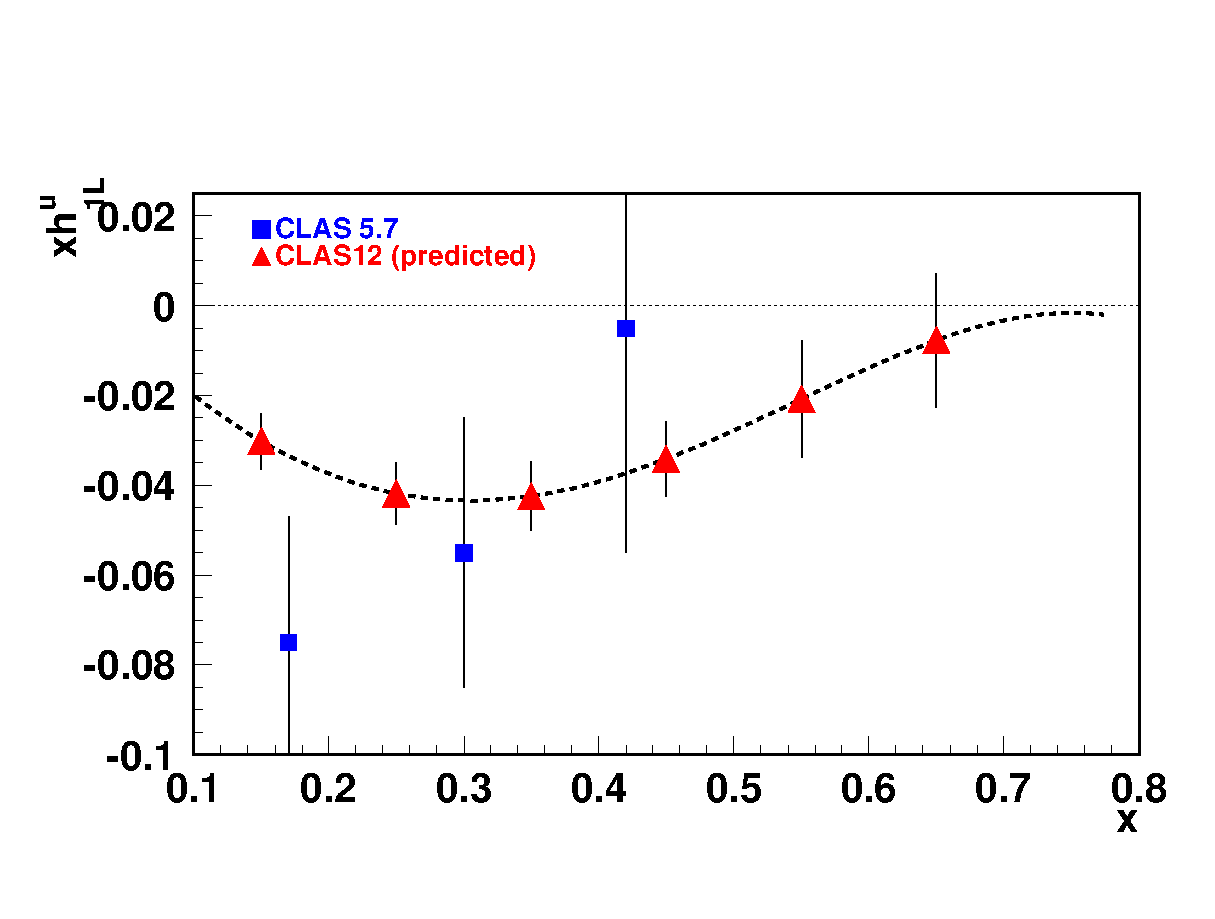
\includegraphics[height=.31\textheight,width=0.45\textwidth]{../sidis/h1lu11.eps}
\\
(a) & (b)
\end{tabular}
\caption{\small{(Left) The projected $x$-dependence of the target SSA at 
11~GeV.  The triangles illustrate the expected statistical accuracy.  The open 
squares and triangles show the existing measurement of the Mulders TMD from 
HERMES and the {\tt CLAS} 5.7~GeV EG1 data sets, respectively.  The curves 
are calculated using Ref.~\cite{Efremov:2004hz}. (Right) Projection for the
Mulders distribution function for the $u$-quark from the $\pi^+$ SSA from 
{\tt CLAS12} (predicted) compared with the {\tt CLAS} EG1 data set at 
5.7~GeV.}}
\label{fig:aul11.sin2}
\end{figure}
%%%%%%%%%%%%%%%%%%%%%%%%%%%%%%%%%%%%%%%%%%%%%%%%%%%%%%%%%%%%%%%%%%%%%%%%%%%%%

Proposed measurements of SSAs in SIDIS will pin down the corresponding TMD 
distribution and will constrain the ratio of favored to unfavored polarized 
fragmentation functions.  The new data will also allow a more precise test of 
the factorization ansatz and the investigation of the $Q^2$ dependence of  
$\sin 2\phi$, $\sin \phi$, and $\cos \phi$ asymmetries. This will enable us 
to study the leading-twist and higher-twist nature of the corresponding 
observables~\cite{Levelt:1994np,Jaffe:1991ra,Kotzinian:1999dy,Afanasev:2003ze,
Yuan:2003gu,Metz:2004je,Collins:2004nx}.

The Boer-Mulders contribution, being leading twist, is expected to survive at 
higher $Q^2$ and that can be tested at the large $Q^2$ accessible with 
{\tt CLAS12}.  At large transverse momentum, {\it i.e.} 
$P_{h\perp}\gg \Lambda_{\rm QCD}$, the transverse-momentum dependence of the 
various factors in the factorization formula~\cite{Ji:2004wu} may be 
calculated from perturbative QCD.  Following the similar arguments in 
Ji-Qiu-Vogelsang-Yuan~\cite{Ji:2006vf}, the $\cos 2\phi$ azimuthal asymmetry 
has the following behavior at $\Lambda_{\rm QCD}\ll P_{h\perp}\ll Q$,

\begin{equation}
\langle \cos 2\phi\rangle|_{P_{h\perp}\gg\Lambda_{\rm QCD}}\propto
\frac{1}{P_{h\perp}^2} \ .
\end{equation}

When the transverse momentum is compatible with the large-scale $Q$, the above 
results will be modified, because the gluon radiation from the pQCD diagram 
will dominate, and contribute to the azimuthal asymmetry not being suppressed 
by any hard scale.  At $Q^2$ values accessible at JLab ($1.0<Q^2<10$~GeV$^2$), 
however, the reduction of the Boer-Mulders asymmetry due to Sudakov form 
factors arising from soft gluon contributions~\cite{Boer:2001he} is not 
expected to be significant.

Measurement of the $P_T$ dependence of the Boer-Mulders-asymmetry (see 
Fig.~\ref{fig:aucos21mx}) will allow for checking of the predictions of a 
unified description of SSA by Ji and collaborators~\cite{Ji:2004wu,Ji:2006vf} 
and for study of the transition from a non-perturbative to a perturbative 
description.  The $\cos 2 \phi$ asymmetry for semi-inclusive deep inelastic 
scattering in the kinematic regions of {\tt CLAS12} is predicted to be 
significant (a few percent on average) and tends to be larger in 
the small-$x$ and large-$z$ region. The preliminary data from {\tt CLAS} at 
6~GeV indeed indicate large azimuthal moments both for $\cos\phi$ and 
$\cos 2\phi$.

%%%%%%%%%%%%%%%%%%%%%%%%%%%%%%%%%%%%%%%%%%%%%%%%%%%%%%%%%%%%%%%%%%%%%%%%%%%%%
\begin{figure}[htbp]
\vspace{6.9cm}
\special{psfile=../sidis/auucos21mxnew.eps hscale=60 vscale=57 hoffset=50 voffset=-5}
\caption{\small{The $\cos2\phi$ moment (Boer-Mulders asymmetry) for pions
as a function of $x$ and $P_T$ for $Q^2>2$~GeV$^2$ (right) with {\tt CLAS12} 
at 11~GeV from 2000~hours of running.  Values are calculated assuming
$H_1^{\perp u\rightarrow \pi^+}=-H_1^{\perp u\rightarrow \pi^-}$.}}
\label{fig:aucos21mx}
\end{figure}
%%%%%%%%%%%%%%%%%%%%%%%%%%%%%%%%%%%%%%%%%%%%%%%%%%%%%%%%%%%%%%%%%%%%%%%%%%%%%

The combined analysis of the future {\tt CLAS12} data on 
$\langle \cos 2 \phi \rangle$ and of the previous ZEUS measurements in the 
high-$Q^2$ domain (where higher-twist effects are negligible) will provide 
information on the Boer-Mulders function, shedding light on the correlations 
between transverse spin and transverse momenta of quarks.  Significantly 
increasing the kinematic coverage at large $Q^2$ and $P_T$, {\tt CLAS12}
(see Fig.~\ref{fig:aucos21mx}) will map the quark TMDs in the valence region
allowing study of the transition from a non-perturbative description at small 
$P_T$ to a perturbative description at large $P_T$.
 
Measured single and double spin asymmetries for all pions in a large range of 
kinematic variables ($x_B$, $Q^2$, $z$, $P_{\perp}$, and $\phi$) combined with 
measurements with unpolarized targets will provide detailed information on the 
flavor and polarization dependence of the transverse momentum distributions of 
quarks in the valence region, and in particular, on the $x_B$, $z$, and 
$P_{\perp}$ dependence of the leading TMD parton distribution functions of $u$ 
and $d$ quarks.  Such measurements across a wide range of $x$, $Q^2$, and $P_T$ 
would allow for detailed tests of QCD dynamics in the valence region 
complementing the information obtained from inclusive DIS.  They would also 
serve as novel tools for exploring nuclear structure in terms of the quark and 
gluon degrees of freedom of QCD.

\section{Summary}

In summary, with upgraded energy and luminosity, {\tt CLAS12} can study 
single- and double-spin asymmetries, involving essentially unexplored 
chiral-odd and time-odd distributions functions, including transversity
\cite{Ralston:1979ys,Jaffe:1991ra}, Sivers~\cite{Sivers:1990fh,Brodsky:2002cx,
Collins:2002kn,Ji:2002aa}, Boer-Mulers~\cite{Boer:1997nt}, and Collins
\cite{Collins:1992kk} functions, providing detailed information on the quark 
transverse momentum and spin correlations~\cite{Collins:1992kk,Kotzinian:1994dv,
Mulders:1995dh,Brodsky:2002rv,Jaffe:2002pj}.

Measurements of semi-inclusive processes combined with inclusive and 
exclusive measurements with an upgraded JLab will allow us to study the quark 
structure of the nucleon with unprecedented detail.  Understanding of 
spin-orbit correlations, together with independent measurements related to the 
spin and orbital angular momentum of the quarks, will help to construct a more 
complete picture of the nucleon in terms of elementary quarks and gluons going 
beyond the simple collinear partonic representation.

